\documentclass[a4paper,10pt]{article}
\usepackage[utf8]{inputenc}

% increase margins
\usepackage{fullpage}
\usepackage[left=1in,top=1in,right=1in,bottom=1in,headheight=3ex,headsep=3ex]{geometry}

% this puts two lines between paragraphs and no indent
\usepackage[parfill]{parskip}

% set up colors
\usepackage{array, xcolor}
\usepackage{color,hyperref}
\usepackage{graphicx}

\definecolor{torontoblue}{HTML}{00204E}
\definecolor{linkblue}{HTML}{0000FF}

% define hyperlink style
\hypersetup{colorlinks,breaklinks,
            linkcolor=linkblue,urlcolor=linkblue,
            anchorcolor=linkblue,citecolor=linkblue}


%opening
\title{Weekly Journal}
\author{Leila Uy}



\begin{document}

\maketitle

\section{Work Update}
A large bulk of my week was spent learning AWS, starting my Literature Review Submission, and researching more articles 
\cite{babatunde2019impact, jain2010data, tang2017parallel, tierney2008snow}. 

\subsection{AWS}
Jishnu and I collaborated in starting our first instance on AWS using the free tier t2.micro to familiarize ourselves with 
instance creation and Linux commands. The t2.micro only has one processor so it is not good for parallel processing but 
it helped me with navigating the E2 console. For example, when I was learning about establishing a possible GUI for an 
instance, I discovered that the Security Groups tabs in the console act as a virtual firewall. It uses the rules to 
determine if it should allow traffic into and out of our instance (e.g., RStudio Servers). I created an excel sheet to help 
keep track of instance types we could use to do experiments on. I think m6g.xlarge, m4.xlarge, or c4.xlarge are the best 
starter instance types.

\subsection{Literature Review Submission}
Mrs. Dr. Maddalena showed us some techniques to use for our Literature Review Submission which I used to establish my 
final goal and four trends that I discovered from the articles I have read since the beginning of the session.

\textbf{Research Goal:} I want to create a parallel k-means clustering R package to help create a consistent, accurate, 
and efficient clustering of ecoregions using large spatial data sets. We can use this classification to preform analysis 
on high resolution data sets of North Carolina to determine if there is a significant shifting of ecoregions as a result 
of climate change.

\begin{table}[h!]
\centering
\begin{tabular}{ |p{2.7cm}| |p{2.5cm}| |p{2.5cm}| |p{2.5cm}| |p{2.5cm}| }
    \hline
    \multicolumn{5}{|c|}{Article Trends} \\
    \hline
    Source & Climate change and ecoregions & Ecoregion consistency &  Parallel programming & Clustering efficency/accuracy \\
    \hline
    Kumar et al. & \_ & X & X & \_ \\
    \hline
    Ellis et al. & \_ & X & \_ & \_ \\
    \hline
    Olson et al. & \_ & X & \_ & \_ \\
    \hline
    Pathak et al. & X & \_ & \_ & \_ \\
    \hline
    Hofierka et al. & \_ & \_ & X & \_ \\
    \hline
    Khan et al. & \_ & \_ & \_ & X \\
    \hline
    Alguliyey et al. & \_ & \_ & X & \_ \\
    \hline
    Pourahmad et al. & \_ & X & \_ & \_ \\
    \hline
    Global Eco. & X & \_ & \_ & \_ \\
    \hline
    Hargrove et al. & \_ & X & \_ & X \\
    \hline
    Luke et al. & \_ & \_ & X & \_ \\
    \hline
    Gbadamosi et al. & X & \_ & \_ & \_ \\
    \hline
    Tang et al. & \_ & \_ & X & X \\
    \hline
    Jain & \_ & \_ & \_ & X \\
    \hline
\end{tabular}
\caption{Literature Review Synthesis}
\end{table}

\textbf{Trends:}
\begin{itemize}
    \item Climate change is affecting agriculture and causing shifts in eco-regions
    \item No consistent and replicable classification of determining eco-regions
    \item Parallel programming makes analysis (e.g., k-means) of big data faster
    \item Clustering can be made more accurate and efficient
\end{itemize}

\section{Literature Review}
60 years after k-means clustering was established, it is still one of the most popular clustering algorithms, but several 
problems arise from clustering and as a result, several extensions of k-means clustering are created. For example, there is 
the Fuzzy cmeans which allows each data point to be a member of multiple clusters using membership value. Different clustering 
algorithms will often result in different partitions, so it is important to choose an algorithm that suits our purpose.
\cite{jain2010data}.  

\begin{figure}[h!]
    \caption{Result of several clusterings of fifteen patterns in two dimensions from Jain 2010 \cite{jain2010data}}
    \centering
    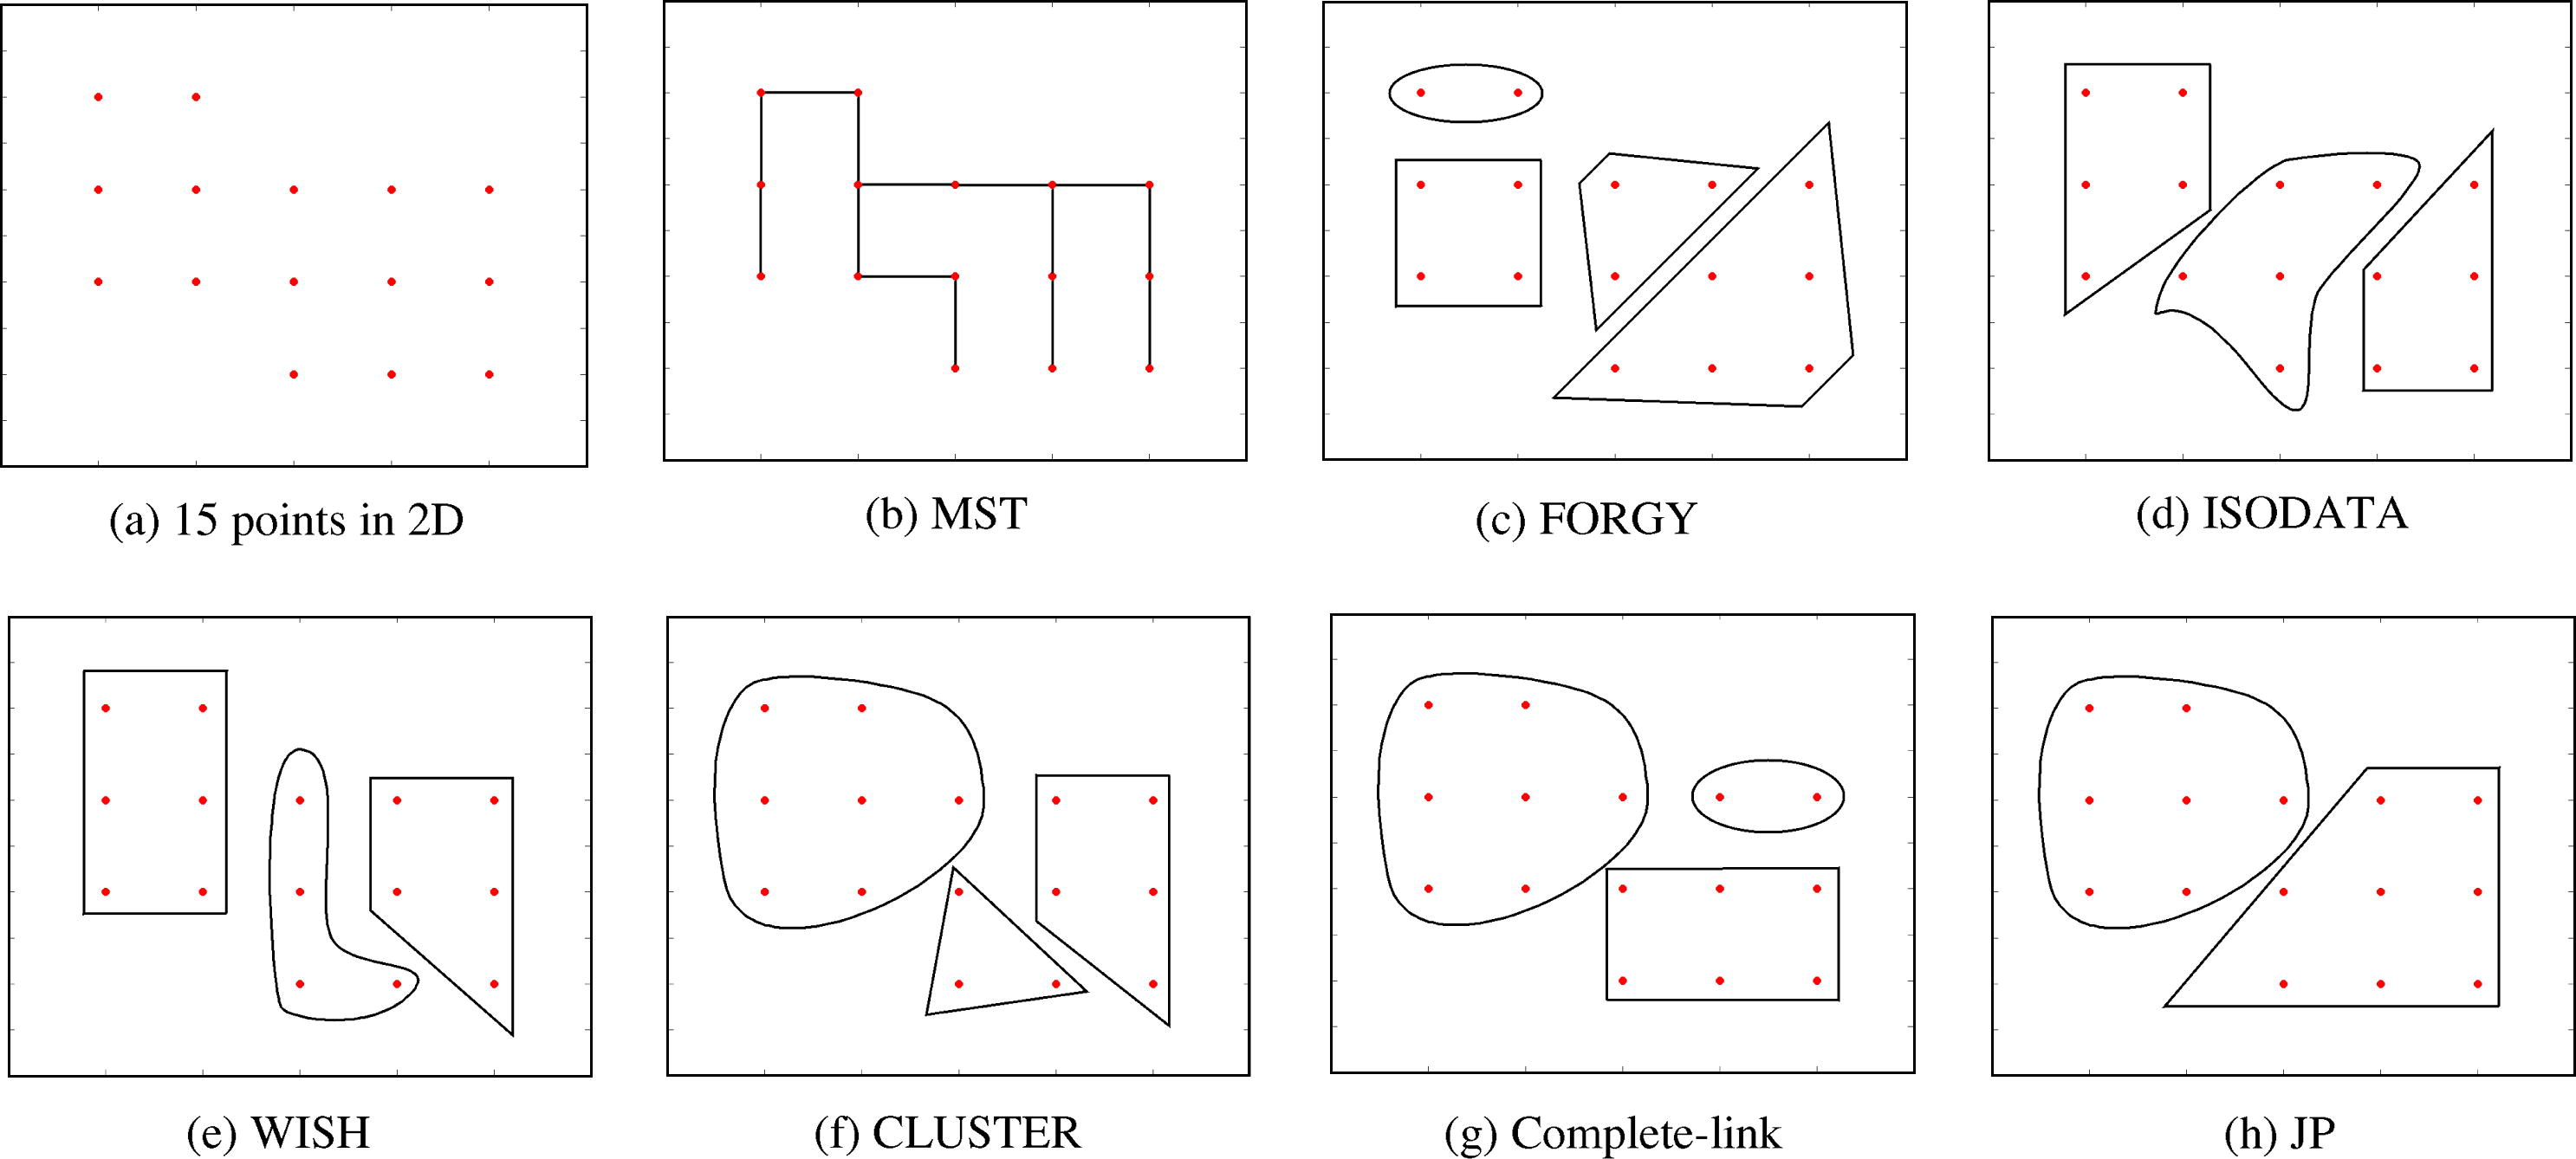
\includegraphics[scale=0.7]{clustering_differences.jpg}
\end{figure}

For my research goal, I want to determine changing eco-regions using large data sets. As we progress technologically, our data 
grows in size and cause problems for iterative algorithms like k-means clustering which will exponentially increase in time 
complexity. Therefore, we want to create an efficient and consistent parallel R program. \cite{tierney2008snow} An article by Tang et al. 
proposed a similar algorithm to Kumar by proposing an elimination of unnnecessary calculations through triangular inequality. 
This article set out to prove this theory using mathematical proofs and proved that extreme point distance calculations can be quickened 
by using Manhattan distance. \cite{tang2017parallel}


% this info creates the bibliography
% YOU WILL NEED TO CHANGE THIS PATH TO THE LOCATION OF THE BIB file
\bibliography{./agclimate.bib}
\bibliographystyle{plain}


\end{document}
